\documentclass[12pt]{article}

\usepackage{booktabs}
\usepackage{tabularx}
\usepackage{hyperref}
\usepackage{graphicx}
\usepackage[a4paper, margin=0.75in]{geometry}
\usepackage{subcaption}
\usepackage{float}


\hypersetup{
    colorlinks=true,       % false: boxed links; true: colored links
    linkcolor=red,          % color of internal links (change box color with linkbordercolor)
    citecolor=green,        % color of links to bibliography
    filecolor=magenta,      % color of file links
    urlcolor=cyan           % color of external links
}

\title{Hazard Analysis\\\progname}

\author{\authname}

\date{}

%% Comments

\usepackage{color}

\newif\ifcomments\commentstrue %displays comments
%\newif\ifcomments\commentsfalse %so that comments do not display

\ifcomments
\newcommand{\authornote}[3]{\textcolor{#1}{[#3 ---#2]}}
\newcommand{\todo}[1]{\textcolor{red}{[TODO: #1]}}
\else
\newcommand{\authornote}[3]{}
\newcommand{\todo}[1]{}
\fi

\newcommand{\wss}[1]{\authornote{magenta}{SS}{#1}} 
\newcommand{\plt}[1]{\authornote{cyan}{TPLT}{#1}} %For explanation of the template
\newcommand{\an}[1]{\authornote{cyan}{Author}{#1}}

%% Common Parts

\newcommand{\progname}{Software Engineering} % PUT YOUR PROGRAM NAME HERE
\newcommand{\teamname}{EvENGage}
\newcommand{\authname}{Team 4, \teamname
\\ Virochaan Ravichandran Gowri
\\ Omar Al-Asfar
\\ Rayyan Suhail
\\ Ibrahim Quraishi
\\ Mohammad Mahdi Mahboob} % AUTHOR NAMES

\newcommand{\prjdesc}{MES Event Management Registration, Administration, and Survey Analytics}

\usepackage{hyperref}
    \hypersetup{colorlinks=true, linkcolor=blue, citecolor=blue, filecolor=blue,
                urlcolor=blue, unicode=false}
    \urlstyle{same}



\begin{document}

\maketitle
\thispagestyle{empty}

~\newpage

\pagenumbering{arabic}

\begin{table}[hp]
\caption{Revision History} \label{TblRevisionHistory}
\begin{tabularx}{\textwidth}{llX}
\toprule
\textbf{Date} & \textbf{Developer(s)} & \textbf{Change}\\
\midrule
09-24-2025 & All members & Brainstorm and Discussion\\
09-24-2025 & Virochaan Ravichandran Gowri & Section 1,2,4\\
09-25-2025 & Rayyan Suhail & Added Component Overview and Boundaries\\
09-29-2025 & Rayyan Suhail & FMEA Added\\
10-07-2025 & Rayyan Suhail, Virochaan Ravichandran Gowri  & Section 6,7 + Review\\
10-07-2025 & All members & Reflection\\
... & ... & ...\\
\bottomrule
\end{tabularx}
\end{table}

~\newpage

\tableofcontents

~\newpage

\pagenumbering{arabic}
\section{Introduction}
This document will contain the Hazard Analysis for \teamname. \teamname \ is a platform which provides the McMaster Engineering Society with the functionality to create and manage events, surveys and perform other administrative functions. It will allow both admins and users to interact with platform and register for events and complete surveys. For this Hazard Analysis we will be defining hazard as a potential risk situation which can result in or contribute to a mishap. The purpose of this document is to identify potential hazards and develop requirements and measure to help prevent or mitigate the risk posed by these hazards.

\section{Scope and Purpose of Hazard Analysis}
The purpose of this Hazard Analysis is to identify and mitigate potential hazards that could negatively impact the \teamname \ platforms. This includes both technical hazards relating to the design of the system as well as user interaction hazards.


\section{System Boundaries and Components}

The proposed platform will be utilized by the McMaster Engineering Society (MES)
as a centralized event management system and survey feedback collection system.
The system boundary includes all the functionality required to build and render
custom forms, manage event registrations and waivers, check-ins, deliver
notifications, and build analytics dashboards.

\subsection{System Boundaries}

\begin{itemize}
    \item \textbf{In Scope}: Administrator and student web and mobile interfaces,
    form builder and renderer, registration and waiver processing, check-in and QR verification,
    attendee overview dashboard, analytics and reporting, notifications, authentication and authorization,
    and internal data storage.

    \item \textbf{Not Covered}: Third-party services like university single sign-on (SSO),
    third-party email/SMS portals, and payment sites. These are treated as outside dependencies,
    with interactions regulated through integration adapters.

    \item \textbf{Environment}: The system is web-based, compatible with major browsers,
    and supports portable devices (iOS and Android). Its operation requires steady internet connectivity,
    although it offers minimal offline capability for the check-in process.
\end{itemize}

\subsection{Component Overview}

The system can be divided into the following major components for hazard analysis:

\subsubsection{Admin Web Application}
Provides administrators with tools to build forms, configure events, manage attendees, and view analytics.

\subsubsection{End-User Application (Web/Mobile)}
Interface for students to register for events and submit feedback surveys.

\subsubsection{Custom Form Builder and Renderer}
Schema-based system to define and display registration and feedback forms, including branching and conditional logic.

\subsubsection{Registration Form Manager}
Handles the creation and processing of registration forms, ensuring that event-specific data is collected accurately.

\subsubsection{Attendee Overview Dashboard}
Provides administrators with a consolidated view of registrations and attendee details for an event.

\subsubsection{Analytics and Reporting}
Generates data visualizations and exportable reports based on registration and survey responses, enabling event planning and improvement.

\subsubsection{Data Storage Layer}
Stores form schemas, form responses, and attendee information using structured databases and JSON-based storage.

\subsubsection{External Integration Adapters}
Interfaces with required external systems such as university single sign-on (SSO) and email services to support core functionality.




\section{Critical Assumptions}

% \wss{These assumptions that are made about the software or system.  You should
% minimize the number of assumptions that remove potential hazards.  For instance,
% you could assume a part will never fail, but it is generally better to include
% this potential failure mode.}
\begin{itemize}
    \item Users will have stable Internet Access: We are assuming that the user will remain connected to the internet as it will be required for using our application.
    \item Users will use the system as intended: We are assuming that users will be not attempting to use the system maliciously and focus on the relevant use cases for this platform.
\end{itemize}

\section{Failure Mode and Effects Analysis (FMEA)}

The following section provides a breakdown of the Failure Modes and Effects Analysis (FMEA) for the system. Each component is evaluated for potential failures, their impact on system operation, possible causes, methods of detection, and recommended actions. This analysis ensures that hazards affecting event registration, form processing, check-ins, and analytics are identified early and mitigated through targeted safety and reliability requirements.
\begin{figure}[H]
\begin{subfigure}{\textwidth}
    \centering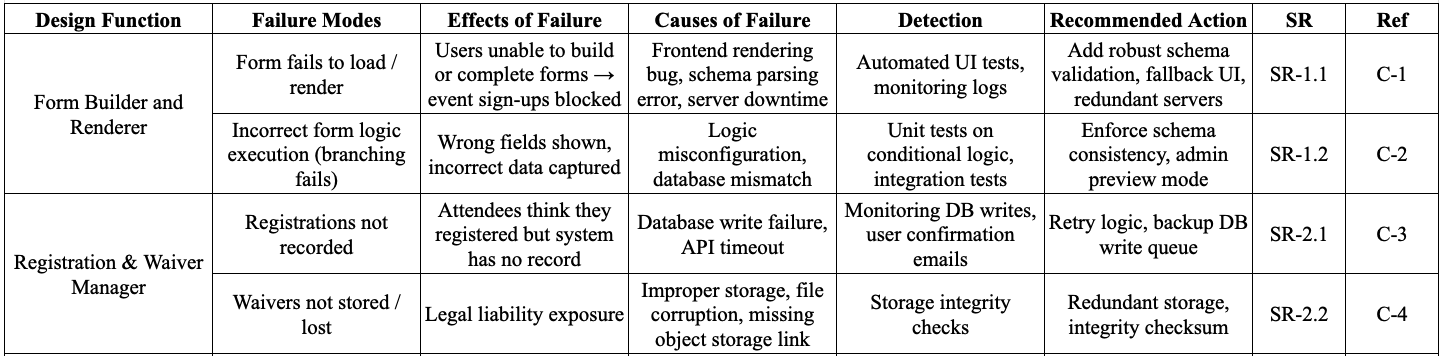
\includegraphics[width=\textwidth]{FMEA_images/FMEA_1.png}
    \caption{Fig. 1: FMEA Table Part 1}
\end{subfigure}

\begin{subfigure}{\textwidth}
    \centering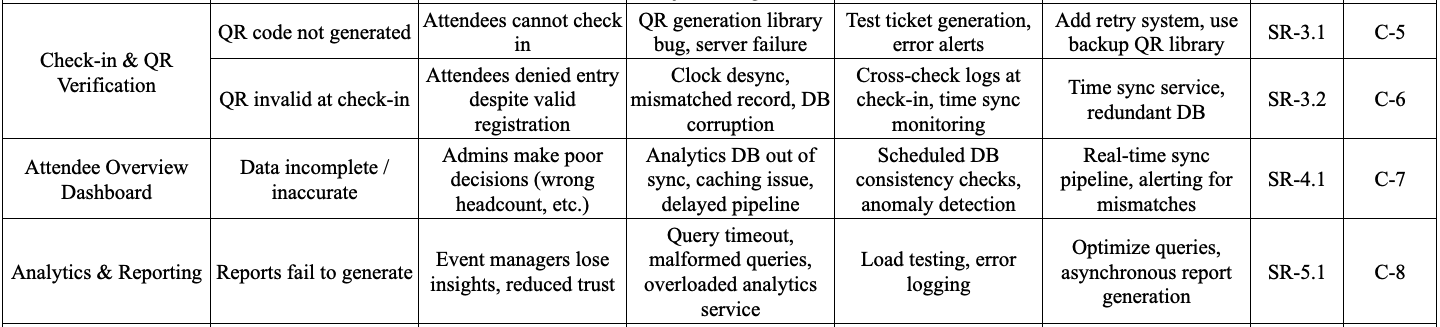
\includegraphics[width=\textwidth]{FMEA_images/FMEA_2.png}
    \caption{Fig. 2: FMEA Table Part 2}
\end{subfigure}

\begin{subfigure}{\textwidth}
    \centering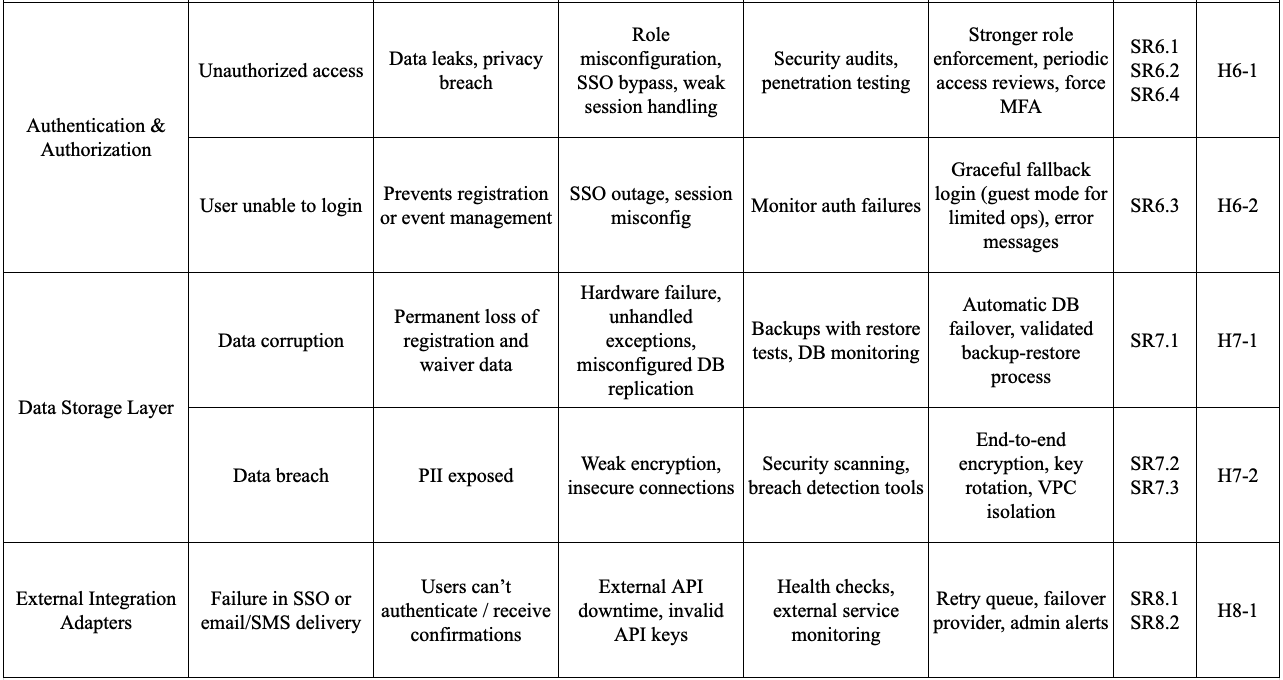
\includegraphics[width=\textwidth]{FMEA_images/FMEA_3.png}
    \caption{Fig. 3: FMEA Table Part 3}
\end{subfigure}
\end{figure}



\section{Safety and Security Requirements}

The following safety and security requirements were derived from the Failure Mode and Effects Analysis (FMEA).
They represent newly discovered requirements that should also be included in the Software Requirements Specification (SRS).

\subsection{Form Builder \& Renderer}
\begin{itemize}
    \item \textbf{SR1.1}: The system shall validate all form schemas before rendering to prevent failures.
    \item \textbf{SR1.2}: The system shall enforce schema consistency across frontend and database logic.
    \item \textbf{SR1.3}: The system shall provide redundant servers or fallback UI during outages.
\end{itemize}

\subsection{Registration \& Waiver Manager}
\begin{itemize}
    \item \textbf{SR2.1}: The system shall implement retry logic and backup queues for database writes.
    \item \textbf{SR2.2}: The system shall send confirmation receipts after successful registration.
    \item \textbf{SR2.3}: The system shall store waiver data redundantly with integrity checks.
\end{itemize}

\subsection{Check-In \& QR Verification}
\begin{itemize}
    \item \textbf{SR3.1}: The system shall provide retry and backup QR code generation.
    \item \textbf{SR3.2}: The system shall enforce synchronized clocks across all check-in endpoints.
\end{itemize}

\subsection{Attendee Overview Dashboard}
\begin{itemize}
    \item \textbf{SR4.1}: The system shall continuously sync databases to prevent inconsistencies.
    \item \textbf{SR4.2}: The system shall implement anomaly detection to detect corrupted or missing data.
\end{itemize}

\subsection{Analytics \& Reporting}
\begin{itemize}
    \item \textbf{SR5.1}: The system shall support asynchronous report generation to handle load.
\end{itemize}

\subsection{Authentication \& Authorization}
\begin{itemize}
    \item \textbf{SR6.1}: The system shall enforce role-based permissions and periodic access reviews.
    \item \textbf{SR6.2}: The system shall support multi-factor authentication for administrators.
    \item \textbf{SR6.3}: The system shall provide a fallback login during SSO outages.
    \item \textbf{SR6.4}: The system shall monitor and log failed login attempts and alert admins.
\end{itemize}

\subsection{Data Storage Layer}
\begin{itemize}
    \item \textbf{SR7.1}: The system shall back up databases automatically and validate restore processes.
    \item \textbf{SR7.2}: The system shall encrypt data at rest and rotate encryption keys regularly.
    \item \textbf{SR7.3}: The system shall store sensitive data in a secure isolated environment (VPC).
\end{itemize}

\subsection{External Integration Adapters}
\begin{itemize}
    \item \textbf{SR8.1}: The system shall implement retry queues and failover providers for external APIs.
    \item \textbf{SR8.2}: The system shall continuously monitor third-party service health and alert admins.
\end{itemize}


\section{Roadmap}

The hazard analysis identified several safety and security requirements. Within the Capstone timeline, the focus will be on core reliability and usability features, including schema validation and fallback UI (SR1.1), reliable registration storage (SR2.1), QR code generation fallback (SR3.1), dashboard synchronization (SR4.1), and authentication fallback handling (SR6.2). More advanced requirements such as multi-factor authentication (SR6.1), scalable analytics (SR5.1), stronger data protection mechanisms (SR7.1, SR7.2), and redundant integration failover (SR8.1) are deferred to future development beyond the Capstone scope. At project completion, the hazard analysis will be revisited to assess which risks have been mitigated and which requirements should be prioritized for follow-up work.


\newpage{}

\section*{Appendix --- Reflection}
% The purpose of reflection questions is to give you a chance to assess your own
learning and that of your group as a whole, and to find ways to improve in the
future. Reflection is an important part of the learning process.  Reflection is
also an essential component of a successful software development process.  

Reflections are most interesting and useful when they're honest, even if the
stories they tell are imperfect. You will be marked based on your depth of
thought and analysis, and not based on the content of the reflections
themselves. Thus, for full marks we encourage you to answer openly and honestly
and to avoid simply writing ``what you think the evaluator wants to hear.''

Please answer the following questions.  Some questions can be answered on the
team level, but where appropriate, each team member should write their own
response:

\subsubsection*{Mohammad Mahdi Mahboob Reflection}
\begin{enumerate}
    \item {\bf What went well while writing this deliverable?}\\
        Identifying the system boundaries was a fairly smooth process. We had already identified most of the items
        listed in this section based on communications with our client. This allowed us to easily and promptly outline
        the items.
    \item {\bf What pain points did you experience during this deliverable, and how did you resolve them?}\\
        Since our solution involves only software interactions and components, there weren't necessarily any imminent
        hazards which were obvious to us when we initially planned this document. I therefore found it a bit difficult
        to conceptualize and appropriately categorize hazards and their severity. After meeting with the TA, we
        had a clearer understanding of the scope which our hazards encompassed, and were able to organize the FMEA and
        create relevant requirement guidelines.
\end{enumerate}

\subsubsection*{Virochaan Reflection}
\begin{enumerate}
    \item \textbf{What went well while writing this deliverable?} \\
    Since we had done work to identify the features and components for the SRS we were able to figure out what could be possible risks that could affect our project. We maintained a heavy emphasis on data privacy since we knew that the application would be collecting sensitive user information. We also talked with our supervisor to see if he had any concerns/risks that we needed to make sure we considered. Overall we identified many risks that could've potentially harmed our projects that we will be looking to mitigate.
    \item \textbf{What pain points did you experience during this deliverable, and how did you resolve them?} \\
    Due to the nature of the project it was hard in the brainstorming stage to actually come up with "hazards" that might actually harm the project in a safety-critical manner. After meeting with our TA we had a better understanding on what we would be considering as a hazard in the scope of this course which allowed us to finish this deliverable.
\end{enumerate}

\subsubsection*{Rayyan Suhail's Reflection}
\begin{enumerate}
    \item \textbf{What went well while writing this deliverable?} \\
    This deliverable went smoothly because our previous documents such as the Problem Statement and Development Plan, gave us a strong foundation to build on. Having already defined the system components helped us structure the hazard analysis efficiently and also the collaboration within the team was smooth, as we divided the sections based on individual strengths. 
    \item \textbf{What pain points did you experience during this deliverable, and how did you resolve them?} \\
    The main challenge we faced was translating general project risks into specific failure modes. Initially, the process felt abstract, but once we began linking each potential failure to real system components (such as form rendering or data storage), it became clearer. Another pain point was determining the appropriate level of detail for each failure mode, we wanted to be detailed without making the table unnecessarily long. We resolved this by focusing on measurable hazards, refining them together as a team. 
\end{enumerate}

\subsubsection*{Omar Al-Asfar Reflection}
\begin{enumerate}
    \item \textbf{What went well while writing this deliverable?} \\
    Defining the safety and security requirements went particularly well since our TA emphasized its importance during our meeting. We had a thorough discussion on how they are often overlooked, and the importance of ensuring that they were actionable and testable. I initially believed this section was going to be lacking since our system is not handling critical or sensitive information, but we were able to come up with a comprehensive list of requirements beyond my expectations.
    \item \textbf{What pain points did you experience during this deliverable, and how did you resolve them?} \\
    The FMEA stood out as a challenging element of this deliverable due to the difficulty in defining failure modes, or explaining how certain risks could manifest as specific failures within our system. However, after our meeting with the TA, we gained clarity on the scope of hazards relevant to our project. This helped us expand on and organize the failures. Once we traced the modes to specific safety requirements and system elements, the analysis became far more manageable.
\end{enumerate}

\subsubsection*{Ibrahim Quraishi Reflection}
\begin{enumerate}
    \item \textbf{What went well while writing this deliverable?} \\
   We found that after completing the problem statement and development plan. Certain sections such as the system boundaries and components were relatively easy to complete. This was due to the problem statement and development plan laying a solid groundwork for defining the main components and scope of the system.
    \item \textbf{What pain points did you experience during this deliverable, and how did you resolve them?} \\
    Defining certain things such as safety-critical hazards was difficult as it did not feel relevant to our system. After further thought and discussions with the TA, we were able to think more critically about the risks that come with similar software systems, such as data leaks. 
\end{enumerate}


\subsubsection*{Group Reflection}
\begin{enumerate}
    \item \textbf{Which of your listed risks had your team thought of before this deliverable, and which did you think of while doing this deliverable? For the latter ones (ones you thought of while doing the Hazard Analysis), how did they come about?} \\
    The primary risks that we identified before the project were what we thought were the obvious ones. Risks relating to the authentication and the data safety during a data breach seemed obvious too us and things that we would have to consider if we were to create any system which had users inputting data. \\
    \\
    Some risks that we thought about through the process of writing this deliverable include the ones relating to data corruption and integrity. This is because these risks are less obvious mainly because all major systems that we use have built in fixes to stop these issues from arising. When we were brainstorming hazards this topic popped up and we realized it was something that we would have to consider to ensure our application worked as intended. Also risks related to the QR code were not really taken into account as we didn't have the prior knowledge on this feature and the risks associated with it. 
    \item \textbf{Other than the risk of physical harm (some projects may not have any appreciable risks of this form), list at least 2 other types of risk in software products. Why are they important to consider?}
    \begin{itemize}
        \item Security/Privacy Risk: We need to ensure that our application is safe from unauthorized data breaches and complies with all privacy regulations. This is important because we want to ensure in our applicaton, whatever information we store is kept secure and it protects us from legal harm as well.
        \item Data Integrity: Data corruption can lead to large losses since it can cause whole databases to fail. This can lead to loss of not just the corrupted data but the whole database itself.
    \end{itemize}
\end{enumerate}

\end{document}


\end{document}

